
We varied the number of gene trees from 5 to 100. We used 20 replicates, estimated gene trees only. From figure \ref{11 Taxon Results-2} we can see that, for all model conditions the rf score of imputed tree is lower than or comparable to that of species tree estimated from incomplete gene trees. For 50-genes and 100-genes, at lower taxa removal rate (9\%-27\%), this score is even lower than that of species tree estimated from complete gene trees. As we increase the taxa removal rate, the rf score for imputed tree goes on to increase. For higher genes (50 and 100), at the highest taxa removal rate (36-45\%) the rf score for imputed tree is comparable to that of incomplete tree. However, for smaller number of genes (5, 15, 25), the rf score for imputed tree shoots up above imputed tree. This can be explained by the Average Dominant Quartet Distribution Match and Mismatch score as shown in figures \ref{fig:Quartet Species Match-11} and \ref{fig:Quartet Species Mismatch-11}. For 5 genes, the match in number of dominant quartets for between Imputed and True species trees falls drastically with that between Incomplete and True species trees with increase in taxa removal rate and goes below the latter for highest rate of taxa removal. This might be because 5 genes contain a very restricted representation of the entire quartet set and removing 36-45\% taxa from this set will remove majority of dominant ones, leaving behind a higher mismatch between dominant quartets between Imputed and True than Complete and True. This mismatch gets amplified by our \textcolor{blue}{IMPUTER} causing the Imputed RF score to increase above that of Incomplete. For 15 and 25 genes at the highest taxa removal rate, the number of matching dominant quartets between Imputed-True is slightly above that of Incomplete-True but still not close to that of Complete-True as seen for lower taxa removal rates, causing Imputed RF score to increase above that of incomplete. For 50 and 100 genes, these problems are not visible and the Imputed RF score is lower than Incomplete RF score for all taxa removal rates.    
\begin{figure}[H]
    \centering
    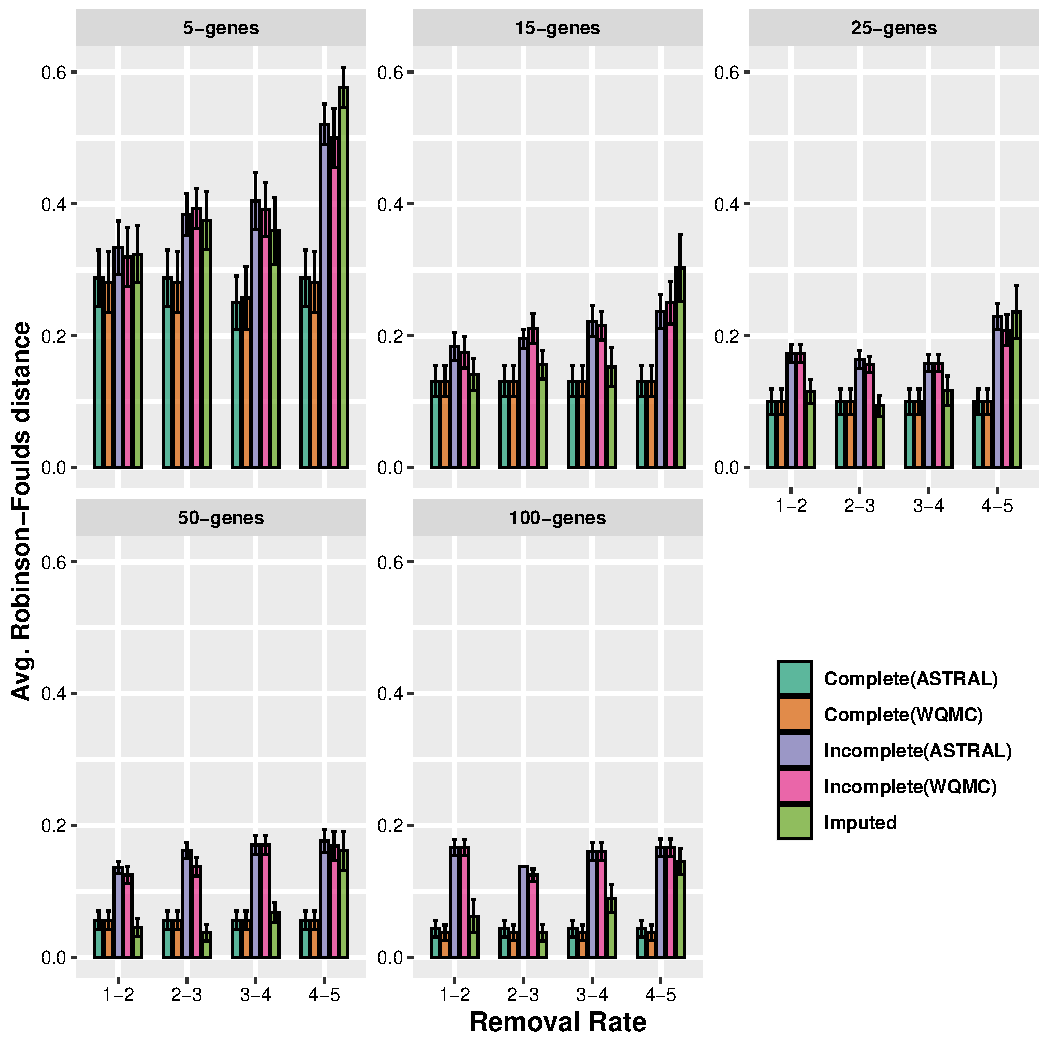
\includegraphics[width=\textwidth]{11_Taxon_Dataset/Result_Images/plot_RF.pdf}
    \caption{Average RF distance of Complete(ASTRAL), Complete(WQMC), Incomplete(Astral), Incomplete(WQMC) and Imputed(WQMC) on the \textbf{11-taxon} dataset with different taxa removal rate. Several taxa removal rate were tried with minimum rate of ($9-18\%$) and a maximum of ($36-45\%$). Only estimated gene trees were analyzed. We show the average RF distance with standard error bars over 20 replicates}
    \label{11 Taxon Results-2}
\end{figure}

\begin{figure}[H]
    \centering
    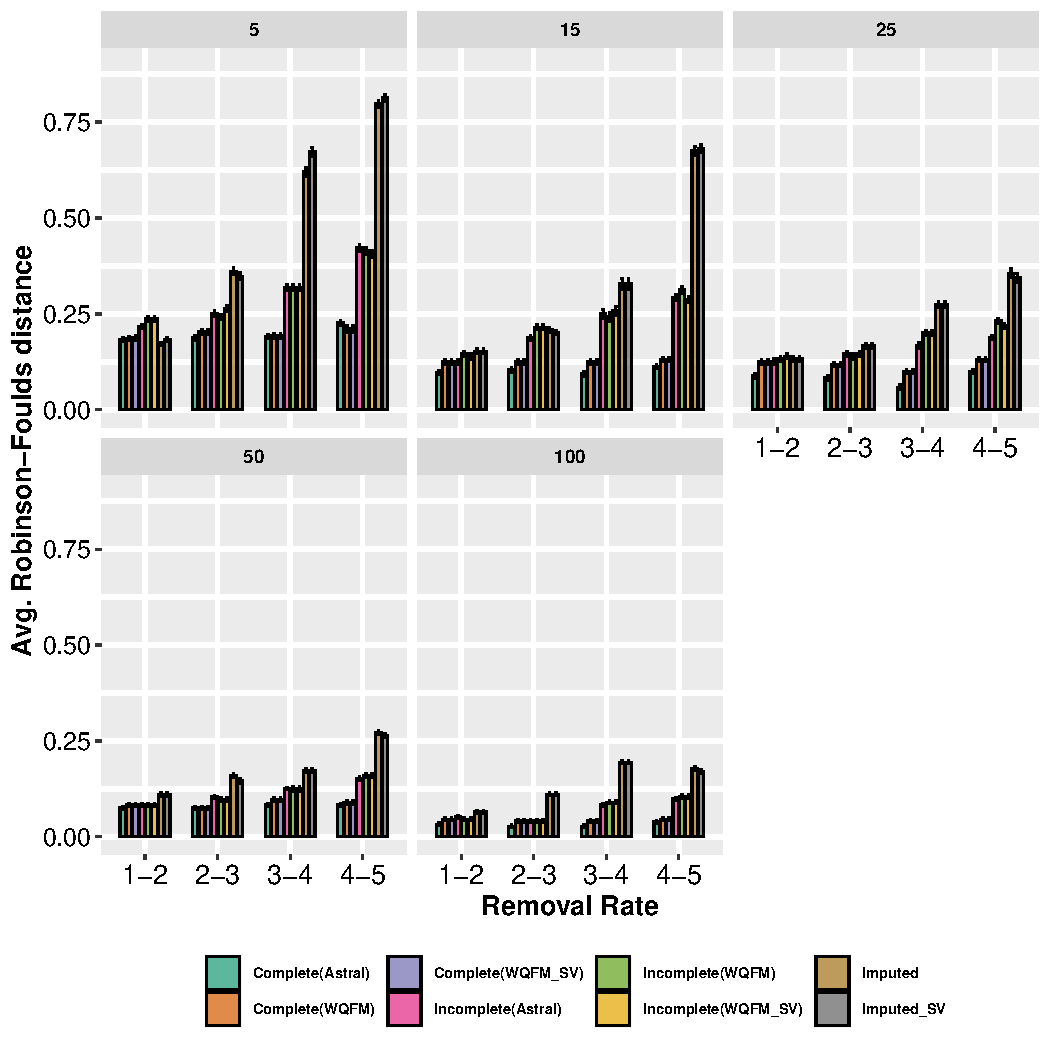
\includegraphics[width=\textwidth]{11_Taxon_Dataset/plot_QRF_WQFM.pdf}
    \caption{Average RF distance of Complete(ASTRAL), Complete(WQFM), Complete(WQFM\_SV), Incomplete(Astral), Incomplete(WQFM), Incomplete(WQFM\_SV), Imputed(WQFM), and Imputed(WQFM\_SV) on the \textbf{11-taxon} dataset with different taxa removal rate. Several taxa removal rate were tried with minimum rate of ($9-18\%$) and a maximum of ($36-45\%$). Only estimated gene trees were analyzed. We show the average RF distance with standard error bars over 20 replicates}
    \label{11 Taxon WQFM RF}
\end{figure}
\begin{figure}[H]
    \centering % <-- added
    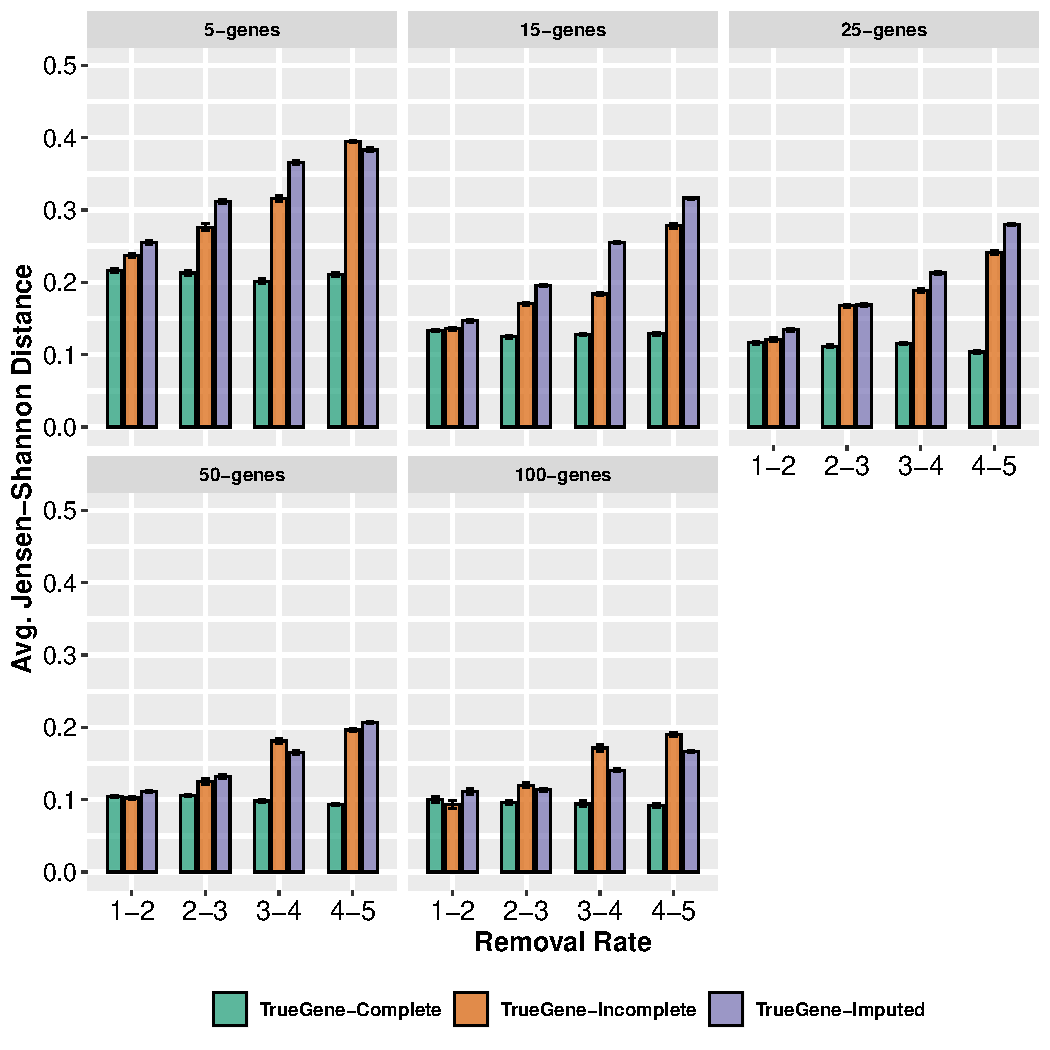
\includegraphics[width=\linewidth]{11_Taxon_Dataset/Result_Images/plot_JSD.pdf}
    \caption{The Jensen-Shannon Distance between the quartet distributions of true gene trees and the complete, incomplete and the imputed gene trees for four taxa removal rate  i.e. 1-2, 2-3, 3-4 and 4-5 taxa respectively.}
    \label{fig:JSD-12}
    \end{figure}
    
\begin{figure}[H]
    \centering % <-- added
    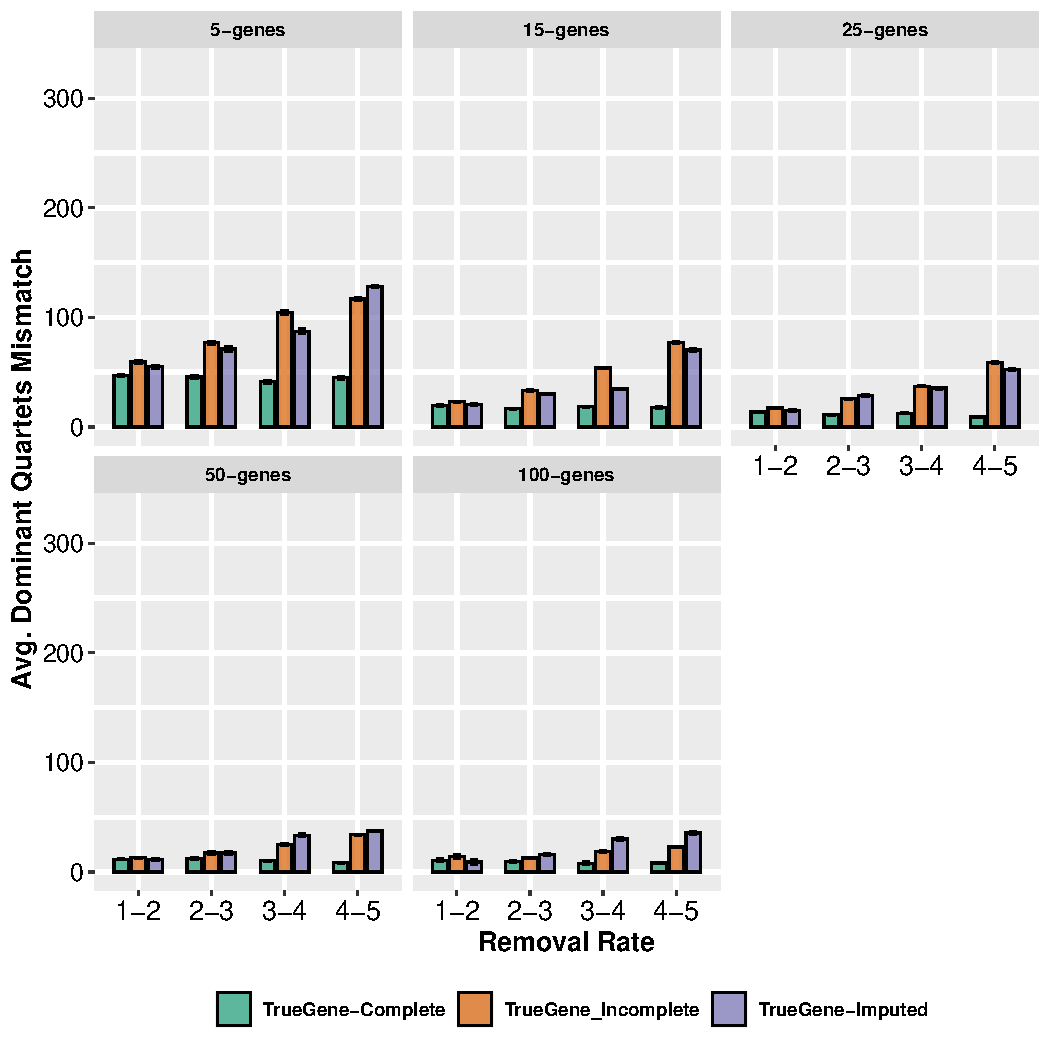
\includegraphics[width=\linewidth]{11_Taxon_Dataset/plot_QM_Gene_Mismatch.pdf}
    \caption{Varying taxa-removal rate, the average quartet distribution mismatch between the true gene quartets and complete, incomplete and imputed gene trees quartets has been shown. The mismatch is higher for the true and incomplete quartet distribution and lowest for the true and imputed one.}
    \label{fig:Quartet Genes Mismatch}
    \end{figure}



\begin{figure}[h]
    \centering % <-- added
    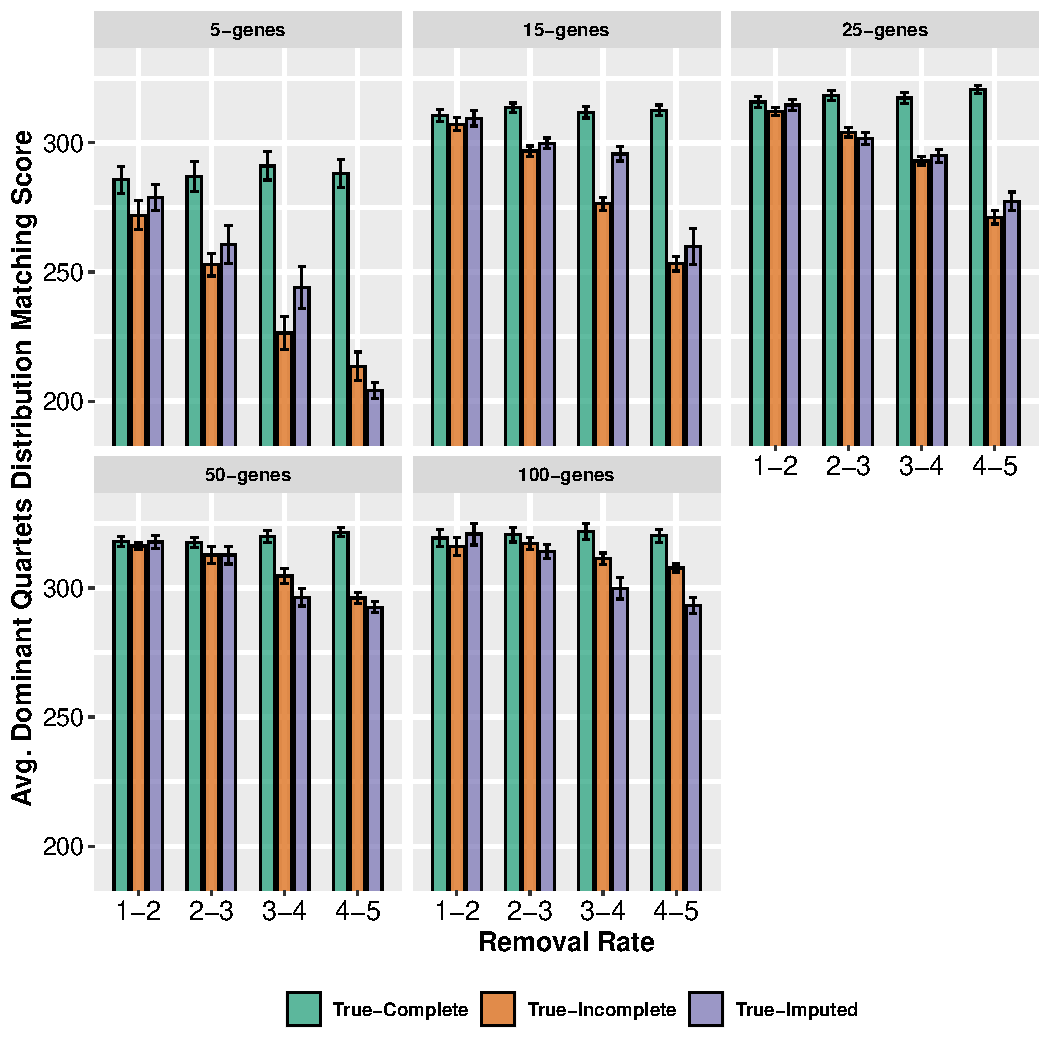
\includegraphics[width=\linewidth]{11_Taxon_Dataset/Result_Images/plot_QM_Species_Match.pdf}
    \caption{Quartets distribution matching between the true species tree quartet and the dominant complete, incomplete and imputed gene trees quartet distribution. They are computed against different taxa removal rate. The average quartet distribution match follow the average robinson-fould distance in most of the cases.}
    \label{fig:Quartet Species Match-11}
    \end{figure}

\begin{figure}[H]
    \centering % <-- added
    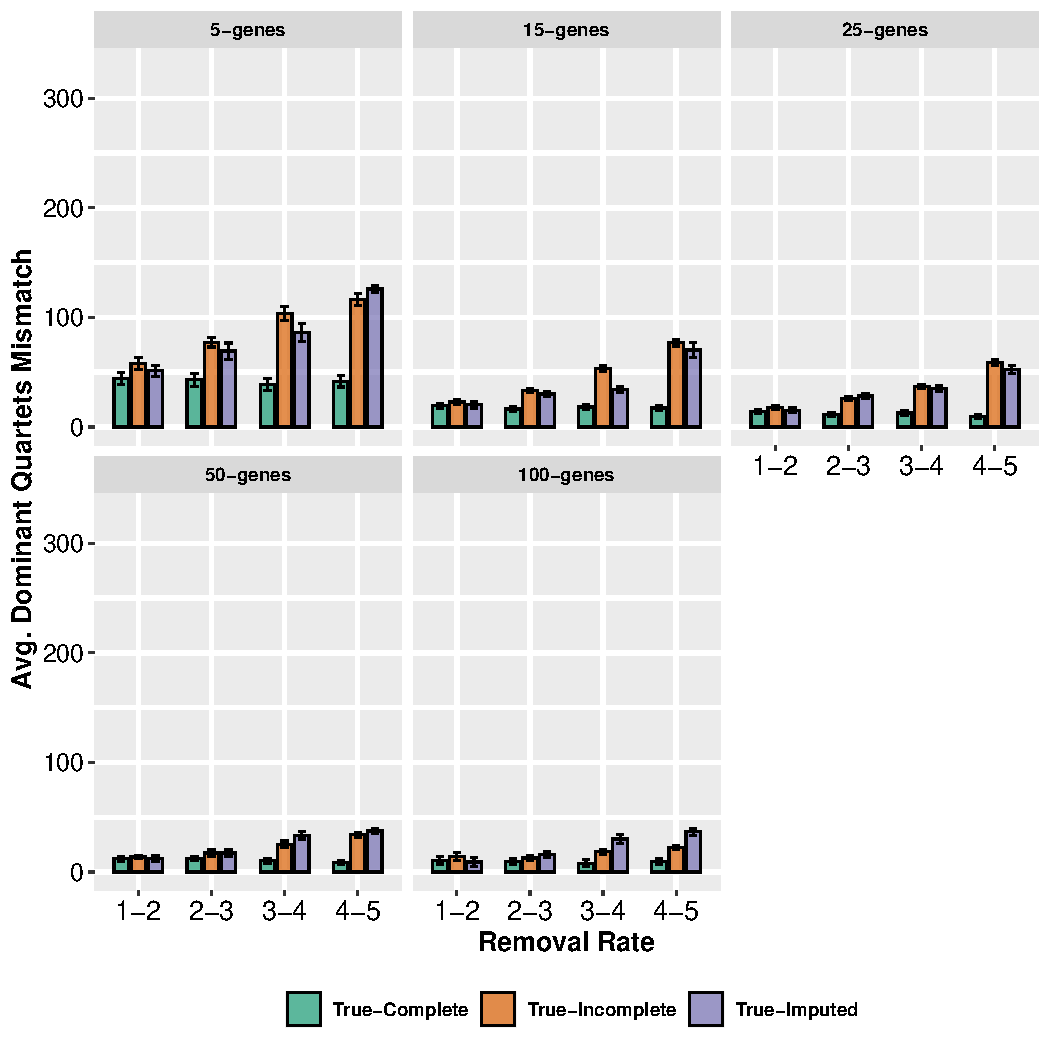
\includegraphics[width=\linewidth]{11_Taxon_Dataset/Result_Images/plot_QM_Species_Mismatch.pdf}
    \caption{Quartets distribution mismatch between the true species tree quartet and the dominant complete, incomplete and imputed gene trees quartet distribution using different taxa removal rate.}
    \label{fig:Quartet Species Mismatch-11}
    \end{figure}


\begin{figure}[H]
    \centering % <-- added
    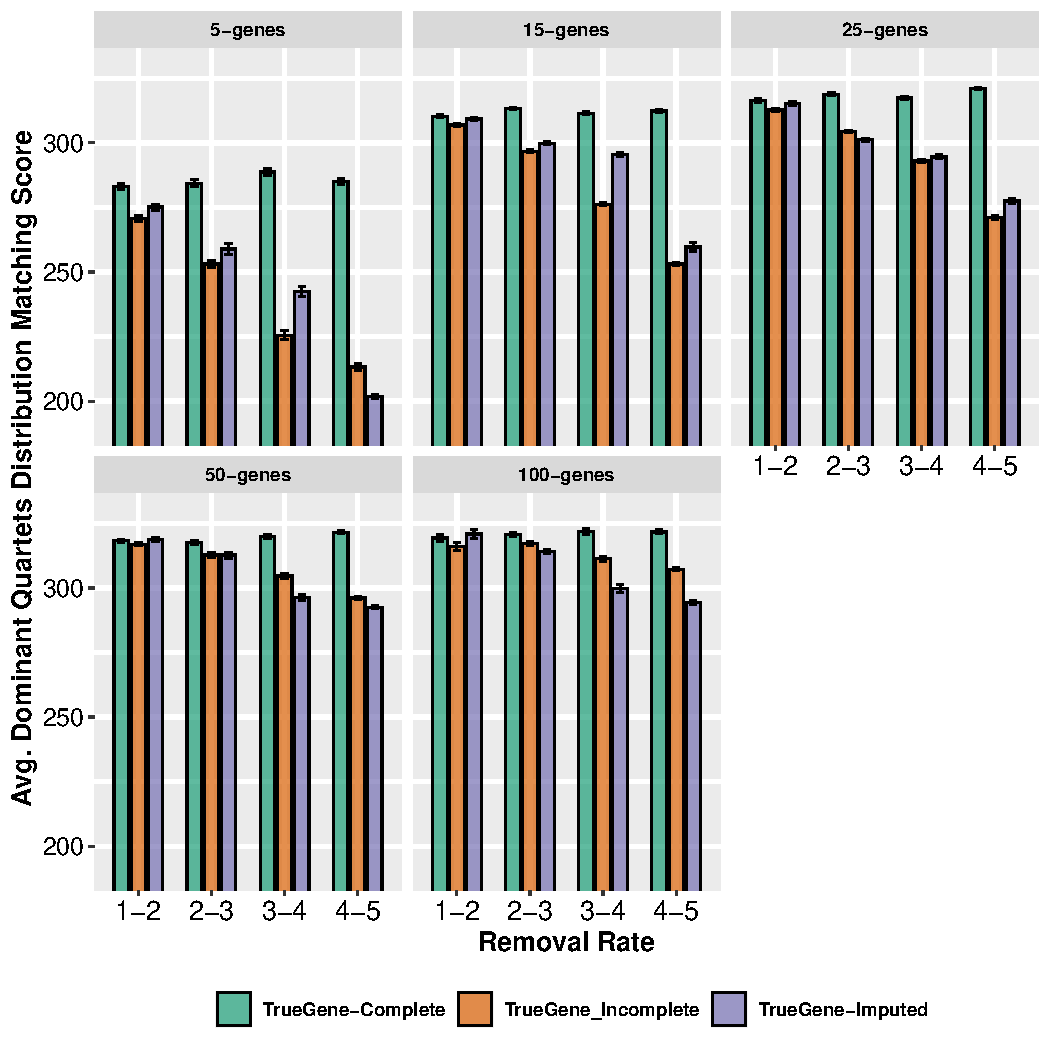
\includegraphics[width=\linewidth]{11_Taxon_Dataset/plot_QM_Gene_Match.pdf}
    \caption{Average quartets distribution matching between the true gene trees quartets and complete, incomplete and imputed quartet distributions.}
    \label{fig:Quartet Genes Match}
    \end{figure}

\paragraph{WQFM Results}
Figure \ref{11 Taxon WQFM RF} shows the results of running WQFM-v2 on complete, incomplete, and imputed quartet sets for 11-taxon dataset. Here Imputed scores appear to be worse than the Incomplete scores instead of making them better. This contradicts the WQMC results reported in Figure \ref{11 Taxon Results-2} which shows that in most cases Imputed scores are better than or comparable to the Incomplete scores. 
%%Subheading -> RF_Rate, Quartets Matching
%%Across all model conditions, the FP is low,so we are better than others here.
%%whiskers (horizontal bar) 
%%grid (only one legend)

